In this section an alloy formulation is provided to model critical aspects of the system. The analysis is mainly focused on the satisfiability of some static constraints, in particular:
\begin{itemize}
	\item it cannot happen that two different users have the same email address.
	\item each city must have at most one municipality, and a municipality is associated to only one city.
	\item authorities have the jurisdiction of only one city, but a city can have multiple registered authorities.
	\item data requests must satisfy the filters.
	\item requested data must be compliant with the user authorization.
\end{itemize}

\vspace{10mm}
\lstinputlisting[language=alloy]{Alloy/Model.als}


\begin{figure}[H]
	\centering
	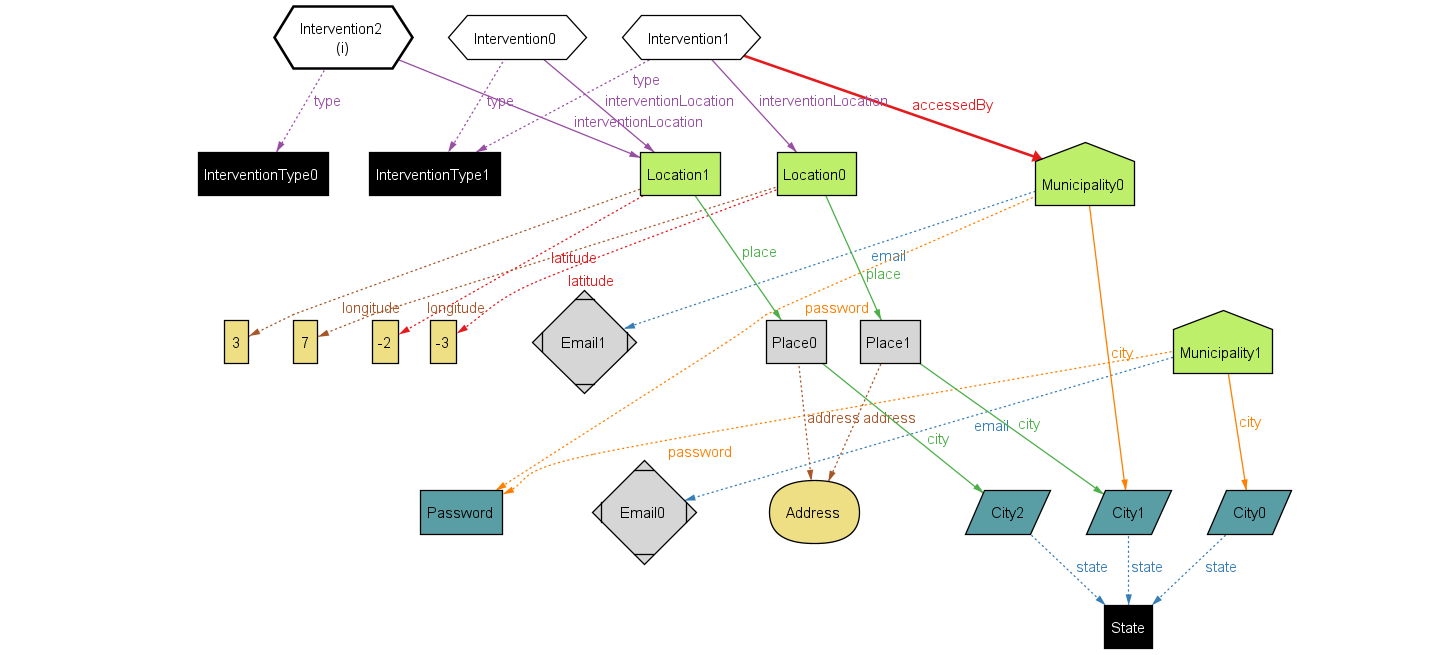
\includegraphics[width=\textwidth]{Alloy/interventionAccessibility}
	\caption{World 3}
\end{figure}

\begin{figure}[H]
	\centering
	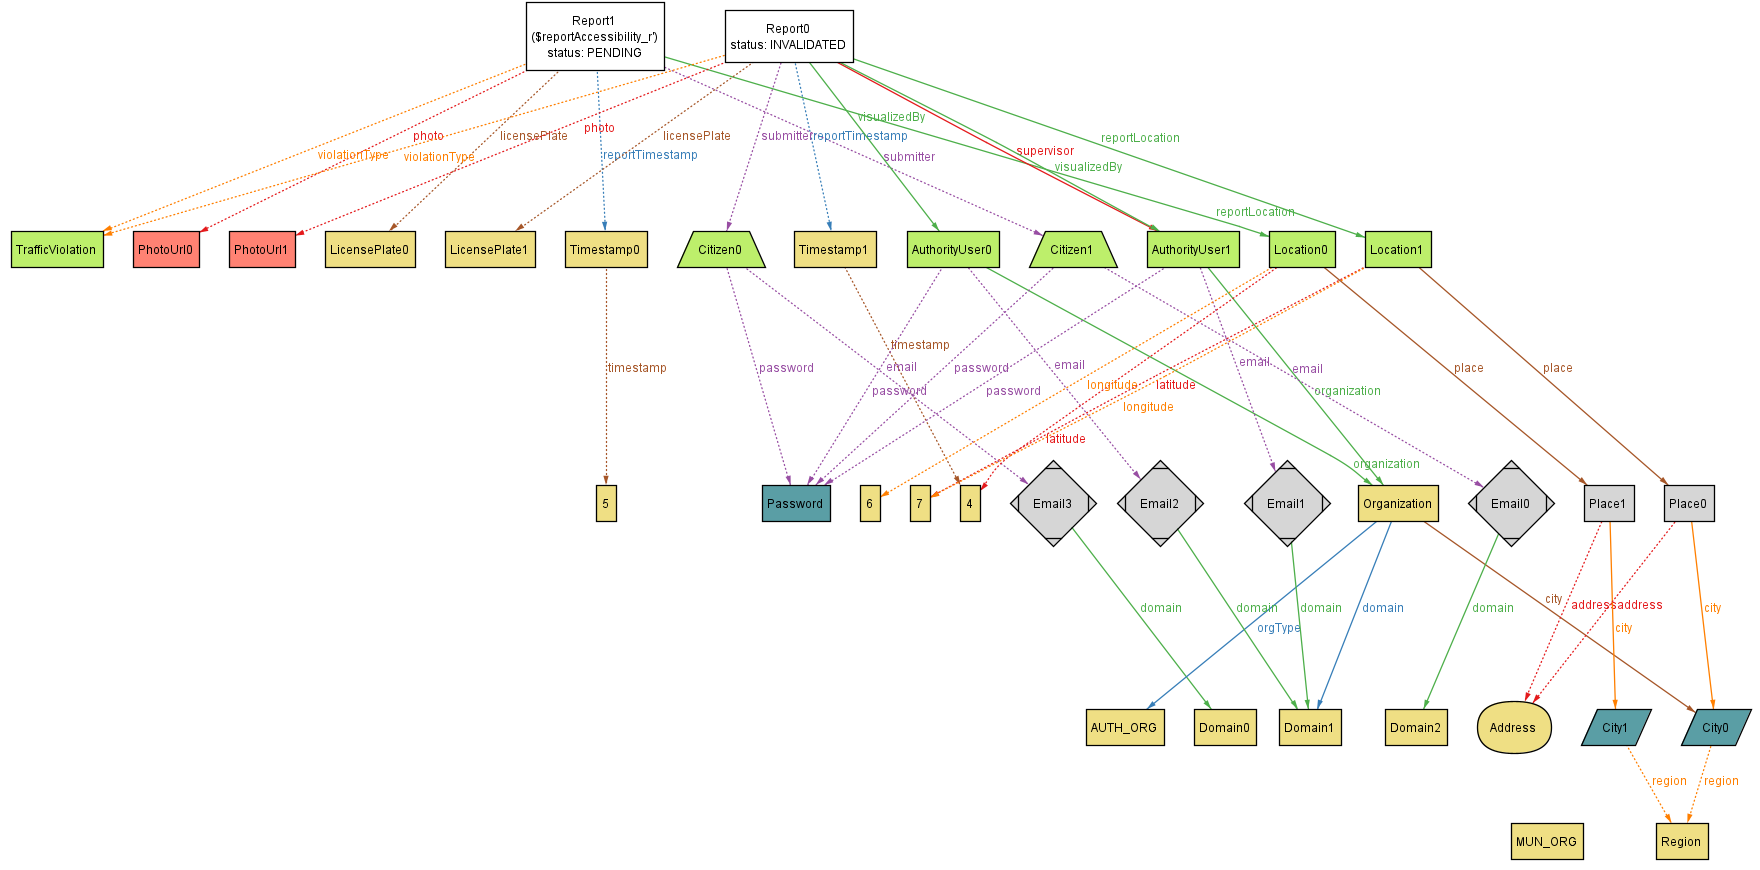
\includegraphics[width=\textwidth]{Alloy/reportAccessibility}
	\caption{World 4}
\end{figure}